Lorem ipsum dolor sit amet, quidam omnesque ea vis. Eum an aliquip legendos recusabo. Mea ex purto natum, ne movet fuisset sit. Labore audiam eos ad, facer ornatus posidonium ne ius, et eos duis delenit nusquam.

\subsection{Project Charter}
The project charter will be based off a SBRI and inform readers of the different aspects of the project. It will cover the details of project background information, cost proposals, team structure, sprint planning, individual status reports, engineering notebooks, and deliverables.

\subsection{Product Backlog}
The Product backlog will include any features that need to be finished at some point in the future. Any new features get added to the backlog and transferred to the sprint backlog at the start of the sprint.

\subsection{Sprint Planning}
Spring planning is detail description of the task that the team members will be doing in a whole sprint cycle. The planning will include goal for a certain period which is usually two weeks, backlog that need to be completed in the cycle is discussed and task breakdown between the team members is done. 

\subsubsection{Sprint Goal}
The sprint goal is the list of the tasks that need to be completed during the sprint cycle. There will be different goals for different spring cycle. Every member of the team will be familiar with the sprint goal.

\subsubsection{Sprint Backlog}
The sprint backlog is a list of tasks that are decided in the sprint meeting and that are to completed during the sprint cycle. The tasks are chosen from the product backlog. The team members keep track of the sprint backlog, which also indicates the progress of the project.

\subsubsection{Task Breakdown}
After the backlog has been decided the tasks are divided between the scrum team members. The division of the task is done in such a way that it will help the scrum team member to meet the sprint goal in timely manner. The main goal of the task breakdown is to break a complex task into simpler and smaller tasks.

\subsection{Sprint Burndown Charts}
Sprint burn down chart is the chart that represents a progress during the sprint cycle. The scrum team is required to have a sprint burn down chart after completion of sprint cycle. This charts will show if the scrum team members are utilizing enough time on the tasks or not. The chart contains an estimated time to complete tasks and actual time spend on those tasks.

\begin{figure}[h!]
    \centering
    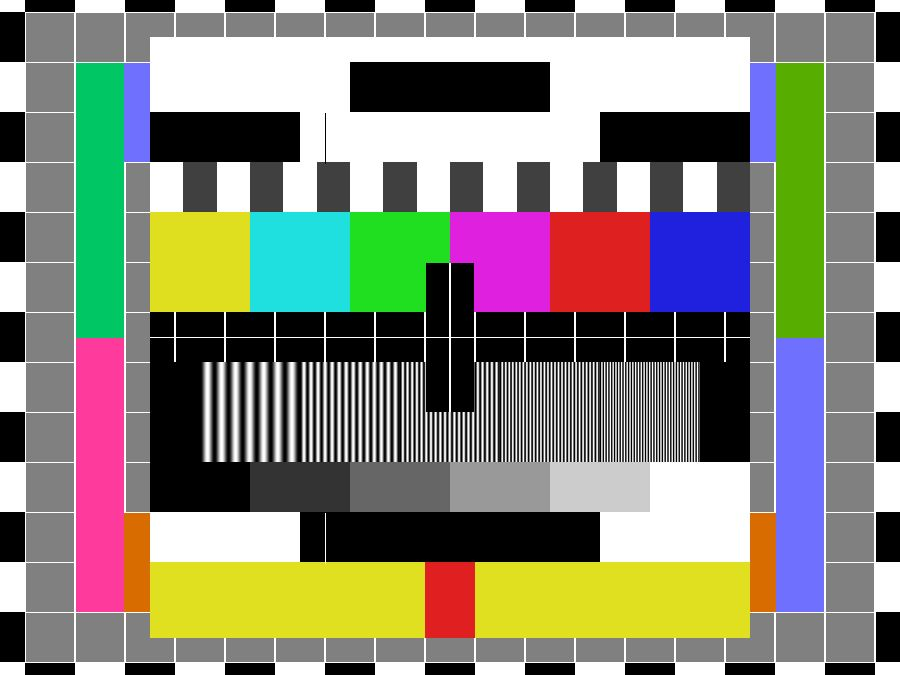
\includegraphics[width=0.5\textwidth]{images/test_image}
    \caption{Example sprint burndown chart}
\end{figure}

\subsection{Sprint Retrospective}
Sprint retrospective is done after every sprint in which whole team participate and discuss about what is working and what is not working. Sprint retrospective is a last thing to work on after completion of the sprint cycle. Things that need to be improved are discussed during the meeting. Product owner, scrum members and scrum master take part in the meeting. 

\subsection{Individual Status Reports}
All the members are required to have this report at the end of the sprint cycle. The main goal of this report is to keep track of team members. In this report team members have to include task they have completed along with time, they have spent and the task they will be working on. Scrum team members are also supposed to include if any other unexpected task appear while completing the given task.

\subsection{Engineering Notebooks}
Engineering notebooks will be used by all team members to record ideas, observations, designs, progress, and what was discussed in team meetings. In addition, the engineering notebook represents official documentation that could be used for patent activities or legal issues. 

\subsection{Closeout Materials}
All the members are required to have this report at the end of the sprint cycle. The main goal of this report is to keep track of team members. In this report team members have to include task they have completed along with time, they have spent and the task they will be working on. Scrum team members are also supposed to include if any other unexpected task appear while completing the given task.

\subsubsection{System Prototype}
The system prototype will consist of a raspberry pi, raspberry pi camera board, pan and tilt brackets, day and night lens, and zoom lens. All of these components will be connected and arranged in an enclosure. 

\subsubsection{Project Poster}
The project poster will contain information regarding the project’s vision, mission, background, and the finished product’s hardware and software details. The poster will be presented at the conclusion of Computer System Design Project II in August, 2016. 

\subsubsection{Web Page}
A web page will be presented to allow the user to view the stream from the camera in a secured manner. They will be allowed to have access with a valid login, password, and IP address. 

\subsubsection{Demo Video}
A demo video will be provided to show how to appropriately use and manage the camera and the software. It will demonstrate all the features of the camera, explain how to view the stream, and describe how to customize the settings in order to fit the needs of the user. The demo video will be delivered through a USB. 

\subsubsection{Source Code}
The source code will consist of software of the user interface to utilize and control the camera. In addition, the source code to allow the user to view the stream of the camera will be provided.  The source code will be delivered in a USB. 

\subsubsection{Source Code Documentation}
The provided source code will be documented properly by including comprehensive comments to allow TrafficNet LLC or their customers to maintain and evolve the software efficiently. The source code documentation will be delivered in a USB. 

\subsubsection{Hardware Schematics}
The design files for the circuit board will be provided to display what was customized in order to attain the appropriate board for the camera. This will be delivered in a USB.

\subsubsection{CAD files}


\subsubsection{Installation Scripts}
The installation scripts of the web page and the firmware for the camera will be provided. The scripts will be delivered in a USB. 

\subsubsection{User Manual}
A user manual will be provided to describe how to properly operate the camera and utilize the software. It will explain in detail the purpose of each feature of the camera and how to appropriately use them. In addition, the manual will describe the software interface and how to make changes according to the user’s preferences. This will be delivered in a USB. 


